\section{Conceitos Básicos}

\subsection{Organização}
Uma entidade social que reúne recursos humanos e materiais com o objetivo de alcançar metas complexas, superando os limites da ação individual.

\subsection{Administração}
Um processo dinâmico que compreende as funções de planejamento, organização, direção e controle, visando utilizar os recursos de uma organização de forma eficaz e eficiente para alcançar seus objetivos e servir à sociedade.

\subsection{Eficácia}
A capacidade de escolher os objetivos mais apropriados e maximizar sua realização. Representa "fazer as coisas certas".

\subsection{Eficiência}
A capacidade de minimizar a utilização de recursos para alcançar os objetivos. Representa "fazer bem as coisas".

\section{Níveis Organizacionais}

Uma organização é tipicamente estruturada em três níveis hierárquicos:

\subsection{Nível Estratégico}
Composto pela alta administração (presidente, vice-presidentes, conselho de administração, etc.). Responsável por definir a missão, visão, objetivos e estratégias da organização como um todo.

\subsection{Nível Tático}
Constituído por gerentes e diretores de unidades de negócio, departamentos ou áreas funcionais. Responsável por traduzir as estratégias definidas pelo nível estratégico em ações concretas para o nível operacional.

\subsection{Nível Operacional}
Composto por supervisores, líderes de equipe e coordenadores de projeto. Responsável pela execução das tarefas e atividades cotidianas da organização.

A importância e a intensidade das funções de administração (planejamento, organização, direção e controle) variam de acordo com o nível hierárquico do gestor. Gestores de nível estratégico dedicam mais tempo ao planejamento, enquanto gestores de nível operacional dedicam mais tempo à direção.

\section{Processo Administrativo}

O processo administrativo consiste em quatro funções interligadas e interdependentes:

\subsection{Planejamento}
Define os objetivos da organização, as estratégias para alcançá-los e os planos que integram e coordenam as atividades da organização.

\subsection{Organização}
Distribui as tarefas e recursos entre os membros da organização, define a estrutura organizacional, a hierarquia e os mecanismos de comunicação e coordenação.

\subsection{Direção}
Relacionada com os processos de liderança, motivação e gestão de pessoas. Busca alinhar os esforços individuais com os objetivos organizacionais.

\subsection{Controle}
Monitora o desempenho da organização para garantir que os objetivos sejam alcançados. Identifica e corrige desvios em relação aos planos.

\section{Áreas Funcionais da Administração}

As organizações se dividem em áreas funcionais especializadas. As principais são:

\subsection{Operações}
Responsável pela gestão das atividades relacionadas à produção de bens ou à prestação de serviços da organização.

\subsection{Marketing}
Responsável por entender e atender às necessidades dos clientes, criando valor para eles por meio de produtos e serviços.

\subsection{Finanças}
Responsável pela gestão dos recursos financeiros da organização, incluindo investimentos, financiamento e controle do fluxo de caixa.

\subsection{Recursos Humanos}
Responsável pela gestão das pessoas na organização, incluindo recrutamento, seleção, treinamento, avaliação de desempenho e remuneração.

\section{Habilidades de um Administrador}

\begin{figure}[H]  % Use H para fixar a posição
    \centering
    \begin{minipage}{0.6\textwidth}
        \centering
        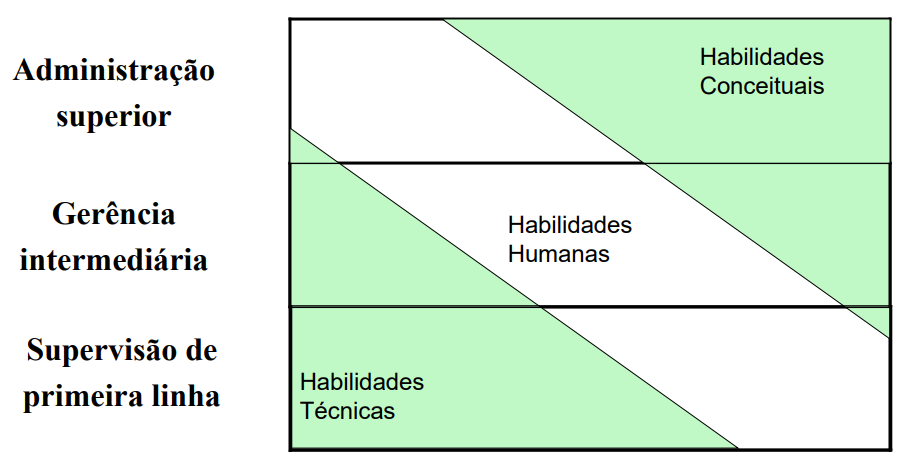
\includegraphics[width=\textwidth]{img/imagem8.png}
        
        \label{fig:exemplo}
    \end{minipage}
\end{figure}

%O texto discute três habilidades importantes para o desempenho de um administrador: \textbf{conceitual}, \textbf{humana} e \textbf{técnica}. A importância de cada habilidade varia de acordo com o nível hierárquico do administrador.

\subsection{Habilidades Conceituais}
\begin{itemize}
    \item Envolvem a capacidade de compreender a complexidade da organização como um todo e o papel de cada parte nesse sistema.
    \item Permitem analisar e interpretar situações abstratas e complexas, facilitando a tomada de decisões mais eficazes e inovadoras.
    \item São essenciais para definir a visão e a estratégia da organização, identificando oportunidades que outros podem não perceber.
    \item São mais relevantes para administradores de \textbf{alto escalão}, que lidam com a organização como um todo.
\end{itemize}

\subsection{Habilidades Humanas}
\begin{itemize}
    \item Referem-se à capacidade de se relacionar, comunicar e compreender as pessoas, motivando-as e liderando-as.
    \item São cruciais para gestores de \textbf{todos os níveis}, pois o trabalho gerencial depende da realização de objetivos por meio de outras pessoas.
    \item Permitem construir um ambiente de trabalho positivo e colaborativo, influenciando a satisfação e o desempenho dos funcionários.
\end{itemize}

\subsection{Habilidades Técnicas}
\begin{itemize}
    \item Envolvem o uso de ferramentas, procedimentos, técnicas e conhecimentos especializados relacionados à área específica de atuação.
    \item São mais importantes em níveis \textbf{operacionais e táticos}, onde o conhecimento específico da área é fundamental para a execução das tarefas.
    \item Para administradores de alto nível, as habilidades técnicas se manifestam no conhecimento profundo da indústria, do mercado e dos processos da organização.
\end{itemize}



% \section{Administração no Brasil}

% A administração no Brasil é influenciada pelo contexto cultural, o que resulta em um estilo de administrar com características próprias.

% \subsection{Sistema de Ação Cultural Brasileiro}
% Um modelo que descreve os impactos da cultura brasileira na administração, com base na relação entre líderes e liderados, e seus subsistemas institucional e pessoal.

% \subsection{Traços Culturais}
% O estilo brasileiro de administrar é marcado por traços como a concentração de poder, a hierarquia, o personalismo, a aversão ao conflito, a flexibilidade, a informalidade e a ênfase em relacionamentos pessoais.

% As empresas brasileiras enfrentam desafios específicos como a elevada carga tributária, a burocracia, os altos custos de financiamento e a baixa produtividade. No entanto, o empreendedorismo, a capacidade de adaptação, a criatividade e a flexibilidade são características que contribuem para o sucesso das empresas no Brasil.
